\documentclass[12pt]{article}
\usepackage{amssymb,amsmath,latexsym, braket,caption, subcaption}
\usepackage{tikz, pgfplots, graphicx, standalone}
\newcommand{\dt}[1]{\frac{\mathrm d #1}{\mathrm dt}}
\renewcommand{\floatpagefraction}{.8}
%\usetikzlibrary{external}
%\tikzexternalize[prefix=i/]
\begin{document}

\title{The Kuramoto Model}
\author{{\bf Supervised Learning Project}\\by\\ {\bf Manish Goregaokar}\\Department of Physics, IIT Bombay\\\quad\\under the guidance of\\{\bf Prof. Punit Parmananda}\\Department of Physics, IIT Bombay }

\maketitle
\begin{center}
\includegraphics[scale=0.25]{i/iitb}
\end{center}

\pagebreak
\stepcounter{section}
\section*{Acceptance letter}
This supervised learning project report titled ``The Kuramoto Model" submitted by Mr. Manish Goregaokar (Roll number 120260006) may be accepted for evaluation.\\

\hfill Professor Punit Parmananda

\hfill \today
\pagebreak
\stepcounter{section}
\section*{Declaration}
 I, Manish Goregaokar, Roll No. 120260006 understand that plagiarism is defined as any one or the combination of the following:
\begin{enumerate}
\item Uncredited verbatim copying of individual sentences, paragraphs or illustrations (such as graphs, diagrams, etc.) from any source, published or unpublished, including the internet.
\item Uncredited improper paraphrasing of pages or paragraphs (changing a few words or phrases, or rearranging the original sentence order)
\item  Credited verbatim copying of a major portion of a paper (or thesis chapter) without clear delineation of who did or wrote what. (Source: IEEE, The Institute,Dec. 2004)
\item I have made sure that all the ideas, expressions, graphs, diagrams, etc., that are not a result of my work, are properly credited. Long phrases or sentences that had to be used verbatim from published literature have been clearly identified using quotation marks.
\item I affirm that no portion of my work can be considered as plagiarism and I take full responsibility if such a complaint occurs. I understand fully well that the guide of the seminar report may not be in a position to check for the possibility of such incidences of plagiarism in this body of work.
\end{enumerate}
\quad
\\\quad
\\Manish Goregaokar
\\Roll No.: 120260006
\\\today\\
\quad\\
{\tiny The above declaration was copied verbatim from http://www.che.iitb.ac.in/online/resources/academic-resources/technical-guides-and-tools/btech-project-btp/declaration-form}
\pagebreak
\stepcounter{section}
\section*{Acknowledgements}
I would like to express my sincere thanks to Professor Punit Paramananda for the opportunity to do this project and his continued guidance. I would also like to express my gratitude towards Tanu Singla, Dinesh Verma, Pawan Dahiya, Shreyans Jain, and Ankit Mahajan for fruitful discussions and inputs during my exploration of the topic.
\pagebreak
\stepcounter{section}
\section*{Abstract}
Synchronization is a common phenomenon occurring with coupled oscillators, where over time their phases become locked. It is observed in a wide range of situations, from the tidal locking of the moon to fireflies to neural clusters. This report gives an overview of this phenomenon, with specific focus on the Kuramoto model.
\pagebreak
\addtocounter{section}{-4}
\tableofcontents\newpage
\section{Introduction}

In 1665, Christiaan Huygens made the first recorded observation and analysis of synchronization\cite{bennett2002huygens}. He noticed that a pair of pendulums kept in the same housing would gradually start moving in unison regardless of their initial conditions. Additionally, if perturbed after the synchronization, the pendulums would re-synchronize. He attributed this effect to the motion of the beam connecting the two, but did not manage to make a complete model of this phenomenon.

The field was quite dormant until the early 1900s, when J. Vincent\cite{vincent1919some}, Van Der Pol\cite{van1920theory}, and E. Appleton\cite{appleton1922automatic} experimented with electrical circuits involving triode oscillators.

After this, there has been a myriad of topics in which synchronization has been studied, including in many electrical, chemical, and biological systems. Additionally, the phenomenon has many applications --- for example, pacemakers are a driving oscillator to the heart in a synchronized system.

\section{Basics}
\subsection{Coupled oscillators}
Systems which individually behave as oscillators can be ``coupled", such that at least one of them is exposed to an effect dependent on the phases of the two oscillators. Usually this effect is monotonic and dependent on the phase difference only. Coupling can be one way or two way ("mutual coupling"). In the one-way case we have a "driving oscillator" which is unaffected by the other oscillator(s), and the other oscillator(s) are known as the "driven oscillator(s)".

For example, for a pair of oscillators, unidirectional coupling could have the equations:
\begin{align*}
\dt{\phi_1} &= \omega \\
\dt{\phi_2} &= \omega - k\sin(\phi_2 - \phi_1)
\end{align*}

whereas bidirectional coupling would be:
\begin{align*}
\dt{\phi_1} &= \omega + k\sin(\phi_2 - \phi_1)\\
\dt{\phi_2} &= \omega - k\sin(\phi_2 - \phi_1)
\end{align*}

In cases where one oscillator has no external effects, sometimes it is considered as ``external forcing".


Oscillators need not have the same $\omega$ (or in general, the same state-space portraits) to be coupled.

\subsection{Synchronization}
Synchronization is simply the process by which a number of coupled oscillators begin to move in lockstep (either in phase or anti-phase) after being allowed to oscillate for some period of time.

For synchronization to happen, the system must be made of coupled oscillators; i.e. the components, when uncoupled, should individually be autonomous oscillators.

A very simple example of synchronization would be where there is a pair of oscillators coupled unidirectionally. It is usually convenient to abstract the driving oscillator away as a "driving force". This makes the system non-autonomous but easier to understand. When the driving force has the same frequency as the oscillator, it is usually guaranteed that there will be phase locking; i.e. the oscillators will eventually have a $0$ or $\pi$ phase difference.

\begin{figure}
\centering
\begin{subfigure}[b]{0.4\textwidth}
\includestandalone[mode=image,width=\textwidth]{i/detuning}
\caption{perfect and imperfect synchronization}\label{fig:detuning}
\end{subfigure}
\begin{subfigure}[b]{0.4\textwidth}
\includestandalone[mode=image,width=\textwidth]{i/arnold}
\caption{Arnold tongue}\label{fig:arnold}
\end{subfigure}
\end{figure}

When the driving force has a different frequency, we have more robust behavior. For low values of the frequency difference, we get \emph{frequency locking} (usually coupled with phase locking) where the driven oscillator eventually oscillates at the driving frequency. However, at higher frequency differences, we no longer have perfect synchronization, however the driven frequency is brought closer to the final one. We can see this behavior in Figure \ref{fig:detuning}, where there is perfect synchronization in a region around $\omega_{\rm driving}$,outside of which the amount of synchronization gradually drops off. The width of this region increases with an increasing driving amplitude. If we plot the region synchronization with amplitude, we get something like Figure \ref{fig:arnold}, known as an \emph{Arnold tongue}\cite{pikovsky2001synchronization}.

Even if the two frequencies are not close, we can still have some synchronization if their harmonics are close. The two frequencies will then attempt to synchronize in a way so that those two harmonics come closer or become equal.
\begin{figure}
\centering
\begin{subfigure}[b]{0.4\textwidth}
\centering
\includestandalone[mode=image,width=\textwidth]{i/almostfull}
\caption{Almost full synchronization}\label{fig:fullgraph}
\end{subfigure}
\begin{subfigure}[b]{0.4\textwidth}
\centering
\includestandalone[mode=image,width=\textwidth]{i/partial}
\caption{Partial synchronization}\label{fig:partialgraph}
\end{subfigure}

\centering
\begin{subfigure}[b]{0.4\textwidth}
\centering
\includestandalone[mode=image,width=\textwidth]{i/nonesync}
\caption{No synchronization}\label{fig:nograph}
\end{subfigure}
\caption{levels of synchronization}
\end{figure}

\subsection{Ensemble of oscillators}

Typically, most synchronizing real systems can be modeled with an \emph{ensemble} of coupled oscillators. Coupling may or may not be global.


In such an ensemble, synchronization can be ``partial"; i.e. there are some elements of synchronization to be found, but it is still not fully synchronized. For example, in Figure \ref{fig:fullgraph}, we have the time series for a system of almost completely synchronized oscillators\footnote{Complete full synchronization would be where the time series for all oscillators are equal or opposite}.

Contrast this with Figure \ref{fig:nograph}, where there is no synchronization at all. While there are times in which the oscillators seem to come close to synchronization, these do not last. However, in Figure \ref{fig:partialgraph}, we have what is known as ``partial synchronization". The majority of the oscillators here are close to the ``mean" time
 series, though there may be a minority of oscillators which are out of phase. It is not necessary that the \emph{same} oscillators will continue to stay somewhat in phase; usually the number of partially synchronized oscillators is approximately constant, however individual oscillators alternate between being in phase and out of phase with the rest.



\section{The Kuramoto Model}
The Kuramoto model was first proposed in 1975 by Yoshiki Kuramoto\cite{kuramoto1975proceedings}
The Kuramoto model models an ensemble of coupled oscillators
$$\dot{\theta_i} = \omega_i + \frac{K}{N}\sum_j a_{ij}\sin(\theta_j - \theta_i) $$

Here, $N$ is the number of oscillators, $K$ is the coupling parameter, and $a_{ij}$ determines how the network of oscillators is coupled. Usually, $a_{ij}=a_{ji}$, and its value is either 0 or 1, denoting uncoupled and coupled oscillators respectively. This matrix defines the topology of the system. Interesting behavior can be observed when the $\omega_i$s are different.

\subsection{Order parameter}
An important way to measure the ``amount" of synchronization. is via something known as the \emph{order parameter}. For an ensemble of oscillators with phases $\theta_i$, the Kuramoto order parameter is 

$$r = \frac1{N}\left|\sum_i e^{i\theta_i}\right|$$

For a completely synchronized system, this parameter is 1, and for an unsynchronized system it will usually be a low value. Partial synchronization is when the value is not small on an average.
\subsection{Computational analysis}
\begin{figure}
\centering
\begin{subfigure}[b]{0.4\textwidth}
\centering
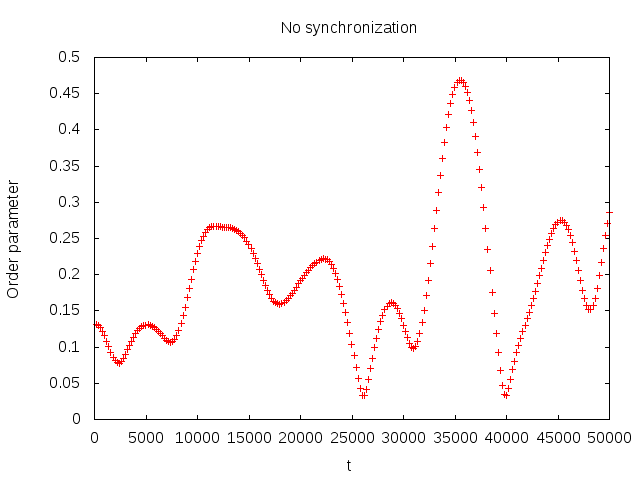
\includegraphics[width=\textwidth]{data/strange}
\caption{No synchronization with $K=0.01$}
\label{fig:plot:nosynchro}
\end{subfigure}
\begin{subfigure}[b]{0.4\textwidth}
\centering
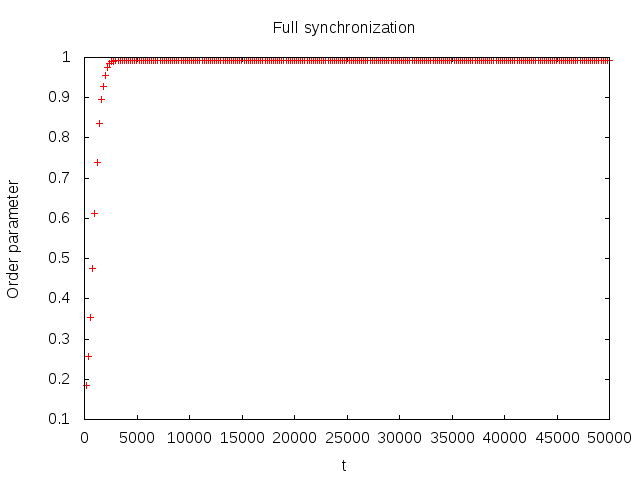
\includegraphics[width=\textwidth]{data/full}
\caption{Full synchronization with $K=0.2$}
\label{fig:plot:full}
\end{subfigure}
\begin{subfigure}[b]{0.4\textwidth}
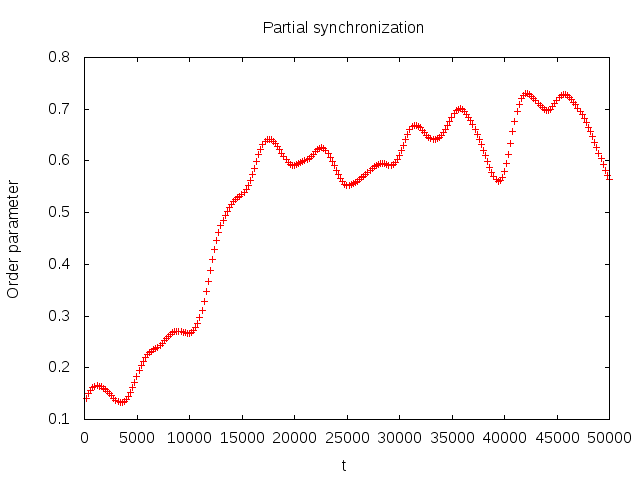
\includegraphics[width=\textwidth]{data/partialsm}
\caption{Partial synchronization with $K=0.05$}
\label{fig:plot:partial1}
\end{subfigure}
\begin{subfigure}[b]{0.4\textwidth}
\centering
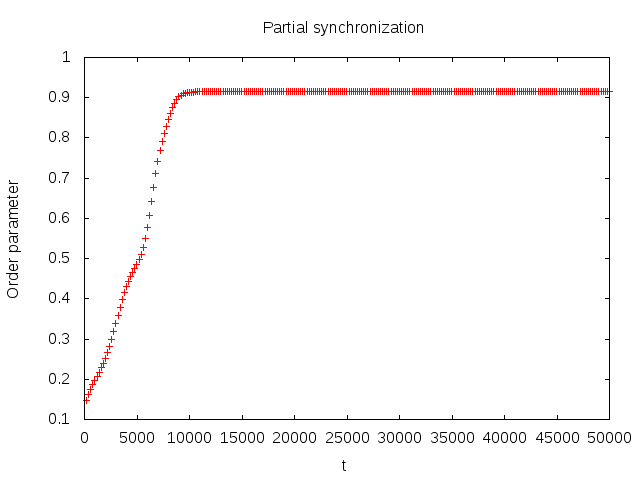
\includegraphics[width=\textwidth]{data/partialmore}
\caption{Partial synchronization with $K=0.07$}
\label{fig:plot:partial2}
\end{subfigure}
\caption{Time series for various levels of coupling}
\end{figure}

I simulated a globally coupled Kuramoto system of 30 oscillators, with a 10\% variation in the $\omega_i$s, and varied $K$. For very low $K$, we get no synchronization as seen in Figure \ref{fig:plot:nosynchro}. While the order parameter may rise to larger values (sometimes even coming close to 1), \emph{on an average} the order parameter stays very low.

While in some cases for partial synchronization the order parameter settles on a particular value and doesn't vary (Figure \ref{fig:plot:partial2}), this is not true in the general case. For example, for lower values of $K$ we can get a time evolution like in Figure \ref{fig:plot:partial1}, where the order parameter doesn't settle, but on an average is an appreciable value. For higher $K$ values, we can have a time evolution similar to that in Figure \ref{fig:plot:partial1}, where the order parameter does settle to a single, large value.


Finally, we can have full synchronization with very large values of the order parameter, as seen in Figure \ref{fig:plot:full}. The ensemble quickly reaches an order parameter of $1$ and stays there.

If we plot the variation of the order parameter with the coupling constant, we get a graph like the one in Figure \ref{fig:plot:ovc}. Note that we have to take a time average of the order parameter (without transients) to get most of the points in this graph since the order parameter for these points is not constant but rather oscillates erratically around some value. Generally, the lower the coupling constant, the more the variation in the order parameter.

\begin{figure}
\centering
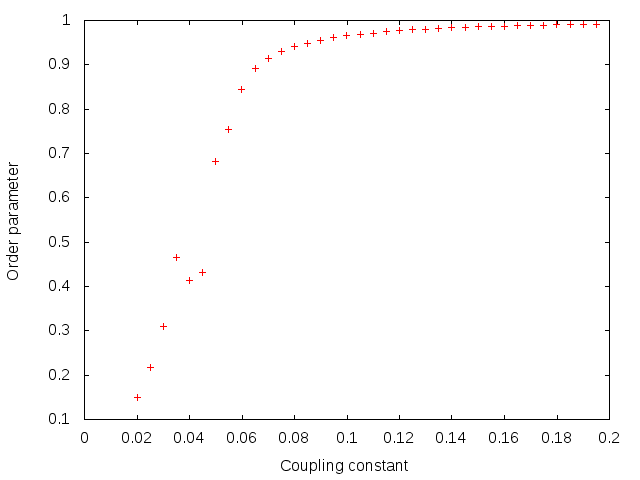
\includegraphics[scale=0.5]{data/ovcoupling}
\caption{Variation of order parameter with coupling constant}
\label{fig:plot:ovc}
\end{figure}
\begin{figure}
\centering
\includestandalone[mode=image]{i/kc}

\caption{Critical coupling}\label{fig:crit}
\end{figure}
Though not very clear in this plot, there is a ``critical coupling strength" (slightly less than 0.02 in this case) $K_c$ beyond which any level of synchronization occurs. Below this, the oscillators act as if they are uncoupled. This can be seen in the theoretical Figure \ref{fig:crit}. The bifurcation observed is a supercritical Hopf bifurcation\cite{niu2014bifurcation}, with the oscillating partially synchronized state bifurcating from the incoherent state.



\subsection{Mathematical analysis}

To be able to get analytical solutions for the model, we must make some reasonable assumptions.
We restrict ourselves to systems where partial to full synchronization occurs, for a large number of oscillators.  Thus, taking the limit $N\to\infty$, and moving to the uniformly rotating frame of the mean phase $\psi$ (We assume it is uniformly rotating). We also only consider cases where the order parameter $r$ is constant (dropping out the situations of partial synchronization where $r$ oscillates around a large average value). This is similar to the mean field model by Winfree\cite{winfree1967biological}
With this in mind, we can rewrite the governing equation as\cite{strogatz2000kuramoto}:

$$\dot\theta_i = \omega_i - Kr\sin{\theta_i}$$

This is a very powerful frame of reference, as now we can actually determine which oscillators will be frequency/phase locked at steady state. Setting $\dot\theta_i = 0$, we get that those oscillators with $|\omega_i| \leq Kr$ will be phase locked at a phase $\theta_i = \sin^{-1}\left(\frac{|\omega_i|}{Kr}\right)$. Note that $\theta_i$ is relative to $\psi$ and $\omega_i$ is relative to $\dot\psi$. Those with $|\omega_i| > Kr$ cannot be phase locked and instead will drift. Its relative angular velocity will vary in a way similar to that shown in Figure \ref{fig:math:drift}
\begin{figure}
\centering
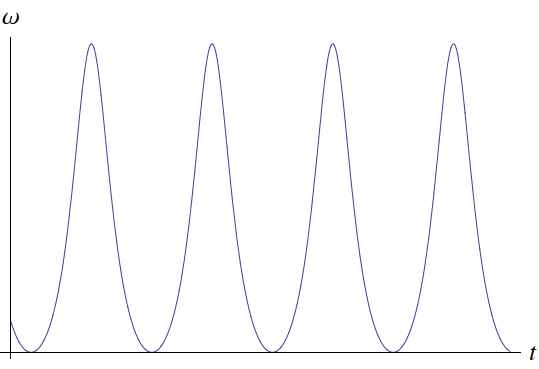
\includegraphics[width=0.7\textwidth]{data/drift}
\caption{Variation of (relative) angular velocity for a drifting oscillator}
\label{fig:math:drift}
\end{figure}

The evolution of the drifting oscillator can be analytically solved as well, giving us 
\begin{align*}
\theta(t) &= 2 \tan ^{-1}\left(\frac{K r+\alpha  \tan \left(\frac{\alpha  t}{2}\right)}{\omega }\right)\\
\dot\theta(t) &= \frac{\alpha ^2 \sec ^2\left(\frac{\alpha  t}{2}\right)}{\omega  \left(\frac{\left(K r+\alpha  \tan \left(\frac{\alpha  t}{2}\right)\right)^2}{\omega ^2}+1\right)}
\end{align*}

where $\alpha = \sqrt{\omega ^2-K^2 r^2}$.

In fact, using this model we can even predict the critical coupling $K_c$ with some additional conditions on the distribution. We must assume that the distribution is ``stationary" (the centroid stays put), and that the distribution of frequencies is symmetric about the mean. Let $g(\omega)$ be the distribution of relative frequencies, and $\rho(\theta,\omega)$ be the distribution of oscillators. The following proof is adapted from one by Stogatz\cite{strogatz2000kuramoto}:
\begin{figure}
\centering
\includestandalone[mode=image]{i/bifur}

\caption{The supercritical Hopf bifurcation of the order parameter}\label{fig:math:bifur}
\end{figure}

Now, we have $r = r_{\rm drift} + r_{\rm lock}$. For the locked oscillators, we have $|\omega|<Kr$, and $\omega=Kr\sin\theta$.

\begin{align*}
r_{\rm lock} &= \int_{-Kr}^{Kr}e^{i\theta}g(\omega)\mathrm d\omega\\
&= \int_{-Kr}^{Kr}\cos\theta g(\omega)\mathrm d\omega\\
&=Kr \int_{-\frac\pi2}^{\frac\pi2}\cos^2\theta g(Kr\sin\theta)\mathrm d\theta
\end{align*}

For the drifting oscillators, we need to consider the distribution of phases too.

\begin{align*}
r_{\rm drift} &= \int_{-\pi}^{\pi}\int_{|\omega|>Kr}e^{i\theta}\rho(\theta,\omega)g(\omega)\mathrm d\omega
\end{align*}
However, this is zero; due to the symmetries $g(\omega)=g(-\omega)$ and $\rho(\theta+\pi,-\omega)=\rho(\theta,\omega)$. The latter symmetry comes because the drifting oscillators must not disturb the centroid on an average.

Thus, we have the equation \begin{align*}
r &=Kr \int_{-\frac\pi2}^{\frac\pi2}\cos^2\theta g(Kr\sin\theta)\mathrm d\theta\\
\implies r &= 0\\
&\text{or} \\
1 &=K \int_{-\frac\pi2}^{\frac\pi2}\cos^2\theta g(Kr\sin\theta)\mathrm d\theta
\end{align*}

The second solution only exists for $K>\frac{2}{\pi g(0)} = K_c$, and we have a supercritical bifurcation for most normal distributions of $g(\omega)$ as shown in Figure\ref{fig:math:bifur}. According to Strogatz\cite{strogatz2000kuramoto}, the bifurcation can be subcritical if $g''(0) < 0$. This is a point on which I intend to do some further investigation in the future.

\section{Applications}
The Kuramoto model has widespread applications. In biology, it can be used to model oscillations of secretory cells, and even synchronization between multiple organisms\cite{winfree1967biological}. Particularly in the field of neurobiology, there are a lot of applications of the Kuramoto model\cite{breakspear2010generative}\cite{cumin2007generalising}. Neural synchronization is conjectured to be a part of visual processing\cite{sompolinsky1991cooperative}, motor coordination\cite{cassidy2002movement}, and memory\cite{klimesch1996memory}, among other things.

This model can be simulated by certain Josephson circuits\cite{wiesenfeld1998frequency}, creating a way to experimentally verify results which cannot be as easily verified with the less reliable (and less tunable) biological systems.

Additionally, it provides a simple approximation for more complex synchronization processes.
\section{Conclusion}
The Kuramoto model is a simple yet robust model of synchronization that applies to a wide variety of processes. It can be analysed in various configurations to attain different results. I myself have started simulating and analysing these configurations, and as shown in the report, have dealt with the basic globally-coupled case. In the future I shall dig deeper into this system by changing the type of coupling and the network used (both scale free and non scale free), as well as compare the explosive Kuramoto case with quorum sensing systems.
\bibliographystyle{abbrv}
\bibliography{bib}
\end{document}

